\documentclass[]{article}
\usepackage{lmodern}
\usepackage{amssymb,amsmath}
\usepackage{ifxetex,ifluatex}
\usepackage{fixltx2e} % provides \textsubscript
\ifnum 0\ifxetex 1\fi\ifluatex 1\fi=0 % if pdftex
  \usepackage[T1]{fontenc}
  \usepackage[utf8]{inputenc}
\else % if luatex or xelatex
  \ifxetex
    \usepackage{mathspec}
  \else
    \usepackage{fontspec}
  \fi
  \defaultfontfeatures{Ligatures=TeX,Scale=MatchLowercase}
\fi
% use upquote if available, for straight quotes in verbatim environments
\IfFileExists{upquote.sty}{\usepackage{upquote}}{}
% use microtype if available
\IfFileExists{microtype.sty}{%
\usepackage{microtype}
\UseMicrotypeSet[protrusion]{basicmath} % disable protrusion for tt fonts
}{}
\usepackage{hyperref}
\hypersetup{unicode=true,
            pdftitle={Supplementary Material: Epigenomic assessment of cardiovascular risk and interactions with traditional risk metrics},
            pdfborder={0 0 0},
            breaklinks=true}
\urlstyle{same}  % don't use monospace font for urls
\usepackage{graphicx,grffile}
\makeatletter
\def\maxwidth{\ifdim\Gin@nat@width>\linewidth\linewidth\else\Gin@nat@width\fi}
\def\maxheight{\ifdim\Gin@nat@height>\textheight\textheight\else\Gin@nat@height\fi}
\makeatother
% Scale images if necessary, so that they will not overflow the page
% margins by default, and it is still possible to overwrite the defaults
% using explicit options in \includegraphics[width, height, ...]{}
\setkeys{Gin}{width=\maxwidth,height=\maxheight,keepaspectratio}
\IfFileExists{parskip.sty}{%
\usepackage{parskip}
}{% else
\setlength{\parindent}{0pt}
\setlength{\parskip}{6pt plus 2pt minus 1pt}
}
\setlength{\emergencystretch}{3em}  % prevent overfull lines
\providecommand{\tightlist}{%
  \setlength{\itemsep}{0pt}\setlength{\parskip}{0pt}}
\setcounter{secnumdepth}{0}
% Redefines (sub)paragraphs to behave more like sections
\ifx\paragraph\undefined\else
\let\oldparagraph\paragraph
\renewcommand{\paragraph}[1]{\oldparagraph{#1}\mbox{}}
\fi
\ifx\subparagraph\undefined\else
\let\oldsubparagraph\subparagraph
\renewcommand{\subparagraph}[1]{\oldsubparagraph{#1}\mbox{}}
\fi

%%% Use protect on footnotes to avoid problems with footnotes in titles
\let\rmarkdownfootnote\footnote%
\def\footnote{\protect\rmarkdownfootnote}

%%% Change title format to be more compact
\usepackage{titling}

% Create subtitle command for use in maketitle
\providecommand{\subtitle}[1]{
  \posttitle{
    \begin{center}\large#1\end{center}
    }
}

\setlength{\droptitle}{-2em}

  \title{Supplementary Material: Epigenomic assessment of cardiovascular risk and
interactions with traditional risk metrics}
    \pretitle{\vspace{\droptitle}\centering\huge}
  \posttitle{\par}
    \author{}
    \preauthor{}\postauthor{}
    \date{}
    \predate{}\postdate{}
  
\usepackage{booktabs}
\usepackage{longtable}
\usepackage{array}
\usepackage{multirow}
\usepackage{wrapfig}
\usepackage{float}
\usepackage{colortbl}
\usepackage{pdflscape}
\usepackage{tabu}
\usepackage{threeparttable}
\usepackage{threeparttablex}
\usepackage[normalem]{ulem}
\usepackage{makecell}
\usepackage{xcolor}

\usepackage{float}

\begin{document}
\maketitle

\newcommand{\beginsupplement}{
  \setcounter{table}{0}  
  \renewcommand{\thetable}{S\arabic{table}}
  \setcounter{figure}{0} 
  \renewcommand{\thefigure}{S\arabic{figure}}
}

\setcounter{table}{0}  
  \renewcommand{\thetable}{S\arabic{table}}
  \setcounter{figure}{0} 
  \renewcommand{\thefigure}{S\arabic{figure}}

\hypertarget{supplemental-methods}{%
\section{Supplemental Methods}\label{supplemental-methods}}

\hypertarget{womens-health-initiative}{%
\subsection{Women's Health Initiative}\label{womens-health-initiative}}

WHI methylation data came from the BA23 ancillary study, a combined
case-control and pseudo case-cohort sampling of 2129 women from the
Women's Health Initiative study. WHI is a larger prospective cohort
beginning in 1993 that included over 160,000 postmenopausal women from
across the United States\textsuperscript{45}. Included subjects had no
self-reported CVD at baseline, and cases were chosen based on incident
centrally adjudicated angina, revascularization, or CHD event during
follow-up. Inclusion criteria for methylation measurement resulted in an
oversampling of African American and Hispanic participants. Blood
samples used for measurement of DNA methylation and clinical
biochemistry were taken at baseline. Data are available in the dbGaP
public repository (accession: phs000200.v11.p3; downloaded on September
27, 2017).

\hypertarget{framingham-heart-study-offspring-cohort}{%
\subsection{Framingham Heart Study Offspring
Cohort}\label{framingham-heart-study-offspring-cohort}}

FHS methylation data came from a substudy of the Framingham Heart Study
that measured DNA methylation in 2726 subjects from the Offspring
Cohort. The Framingham Offspring Cohort was originally established in
1971 to follow 5209 children of the original Framingham Heart Study
participants and their spouses\textsuperscript{46}. Fasting blood samples
for both methylation and clinical biochemistry were collected from
participants at Exam 8, which took place from 2005-8. Blood samples were
also provided for clinical biochemistry measurements in previous exams,
constituting the ``past exposures'' examined here. Data are available in
the dbGaP public repository (accession: phs000007.v29.p10; downloaded on
September 27, 2017). Adjudicated cardiovascular event data was collected
through 2015, and events were defined here as any of: myocardial
infarction, angina pectoris, stroke (approximately 90\% being ischemic),
or death from CHD (Framingham event codes 1-29). FHS methylation data
were collected in two primary batches in two centers -- one in subjects
from a nested case-control for CVD measured at Johns Hopkins University
(FHS-JHU)\textsuperscript{47}, and the other in a larger set of
remaining Framingham Offspring participants measured at the University
of Minnesota (FHS-UM).

\hypertarget{lothian-birth-cohorts}{%
\subsection{Lothian Birth Cohorts}\label{lothian-birth-cohorts}}

The Lothian Birth Cohorts consist of two birth cohorts (born in 1921 and
1936) established in the Lothian region of Scotland\textsuperscript{48,49}. Only the 1936 cohort was analyzed here. Blood samples
were collected in three waves starting in 2004, with our primary
analyses here focusing on samples from Wave 1 (2004-2007).
Cardiovascular outcomes were defined as general CVD or stroke determined
at each wave, and event times for survival models were approximated
based on the time between Wave 1 and the wave at which the event was
reported. LBC data are accessible through the European Genome-phenome
Archive (accession: EGAD00010000604).

\hypertarget{regicor}{%
\subsection{REGICOR}\label{regicor}}

The REGICOR dataset analyzed here consisted of a nested case-control for
myocardial infarction within the larger REGICOR (REgistre GIroní del
COR) cohort from the Girona Province in Catalonia (Spain). Whole blood
samples were collected from 391 total participants, with those from
cases generally collected within 24 hours of the event. Characteristics
for this population are available in Supp. Table S3.

\newpage

\hypertarget{supplemental-tables}{%
\section{Supplemental Tables}\label{supplemental-tables}}

\begin{ThreePartTable}
\begin{TableNotes}
\item[1] No covariates
\item[2] Adjusted for age, sex, and estimated cell type fractions
\item[3] Additionally adjusted for BMI, LDL, HDL, SBP, diabetes status, and current smoking
\item[4] Adjusted for Framingham Risk Score only
\end{TableNotes}
\begin{longtable}[t]{lrl}
\caption{\label{tab:fhs-holdout-noPE}MRS performance in held-out FHS subset without past CVD events}\\
\toprule
Model & HR per s.d. MRS & p\\
\midrule
Unadjusted\textsuperscript{1} & 1.55 & 1.9e-08\\
Basic\textsuperscript{2} & 1.27 & 7.3e-03\\
Plus risk factors\textsuperscript{3} & 1.30 & 6.0e-03\\
FRS only\textsuperscript{4} & 1.37 & 7.7e-05\\
\bottomrule
\insertTableNotes
\end{longtable}
\end{ThreePartTable}

\begin{longtable}[t]{llrr}
\caption{\label{tab:stability}MRS stability as evaluated by using multiple within-subject measurements. Generic ICC heuristics for reference: 0-0.5 = poor, 0.5-0.75 = moderate, 0.75 - 0.9 = good, 0.9-1 = excellent.}\\
\toprule
Cohort & Group type & \# of pairs/groups & ICC\\
\midrule
FHS & Duplicates & 26 & 0.85\\
LBC36 & Samples over multiple visits & 758 & 0.68\\
LBC36 & Samples over subsequent visits (Wave 1 \& 2) & 758 & 0.69\\
LBC36 & Samples over longer time frame (Wave 1 \& 3) & 758 & 0.61\\
\bottomrule
\end{longtable}

\begin{longtable}[t]{ll}
\caption{\label{tab:regicor-description}Description of REGICOR myocardial infarction nested case-control population (continuous variables presented as: mean (standard deviation))}\\
\toprule
Sample size & 391\\
Prior myocardial infarction & 50.1\%\\
Ancestry (\% European) & 100\%\\
Age & 63.2 (6.9)\\
Sex (\% female) & 48.6\\
Smoking & 21.5\%\\
Body mass index & 28.5 (4.8)\\
Hypercholesterolemia & 53.0\%\\
Hypertension prevalence & 57.1\%\\
Diabetes prevalence & 24.7\%\\
\bottomrule
\end{longtable}

\begin{longtable}[t]{lrl}
\caption{\label{tab:risk-score-validation}Validation of Framingham Risk Score}\\
\toprule
Study & HR per s.d. MRS & p\\
\midrule
WHI & 1.50 & 4.7e-61\\
FHS-JHU & 1.40 & 9.9e-06\\
FHS-UM & 1.63 & 8.5e-22\\
LBC & 1.01 & 9.2e-01\\
\bottomrule
\end{longtable}

\begin{longtable}[t]{llr}
\caption{\label{tab:regicor-interactions}Risk factor-stratified MRS performance in the REGICOR dataset}\\
\toprule
Risk factor group & OR per s.d. MRS [95\% CI] & N\\
\midrule
Q1 & 4.49 [1.64-12.28] & 119\\
Q2 & 1.17 [0.67-2.04] & 90\\
Q3 & 2.58 [1-6.68] & 60\\
Q4 & 1.2 [0.31-4.59] & 55\\
\bottomrule
\end{longtable}

\newpage

\hypertarget{supplemental-figures}{%
\section{Supplemental Figures}\label{supplemental-figures}}

\begin{figure}[h]
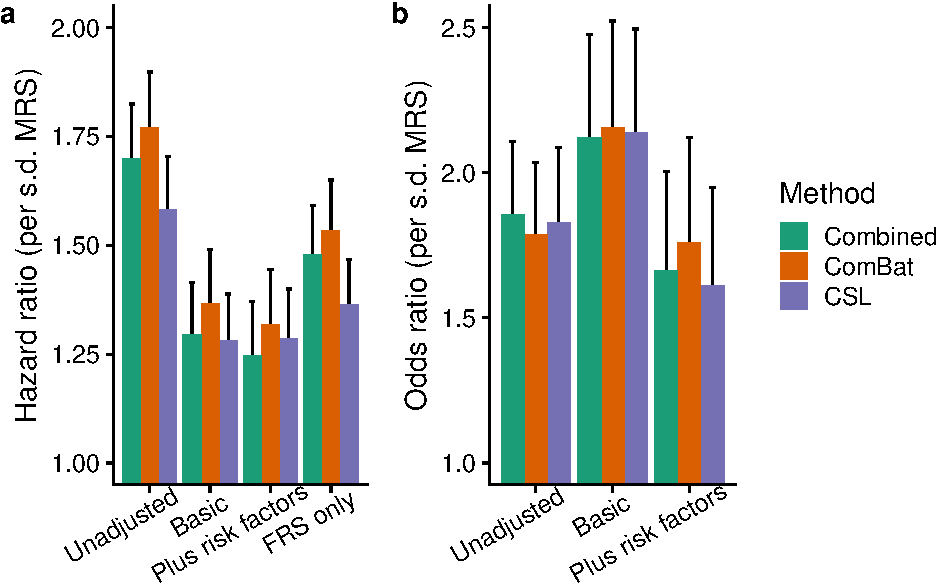
\includegraphics{figures/csl-comparison-1} \caption{Comparison of modeling approaches. Performance metrics are shown as a function of the test dataset, either FHS-UM (a) or REGICOR (b), and the covariate adjustment. Performance is quantified by either hazard ratio from Cox models (a) or odds ratio from logistic models (b). Covariate sets used for adjustment for models named here are identical to their descriptions for the regression models presented above. Errors bars represent standard errors for the hazard ratio or odds ratio estimates.}\label{fig:csl-comparison}
\end{figure}

\newpage

\begin{figure}[h]
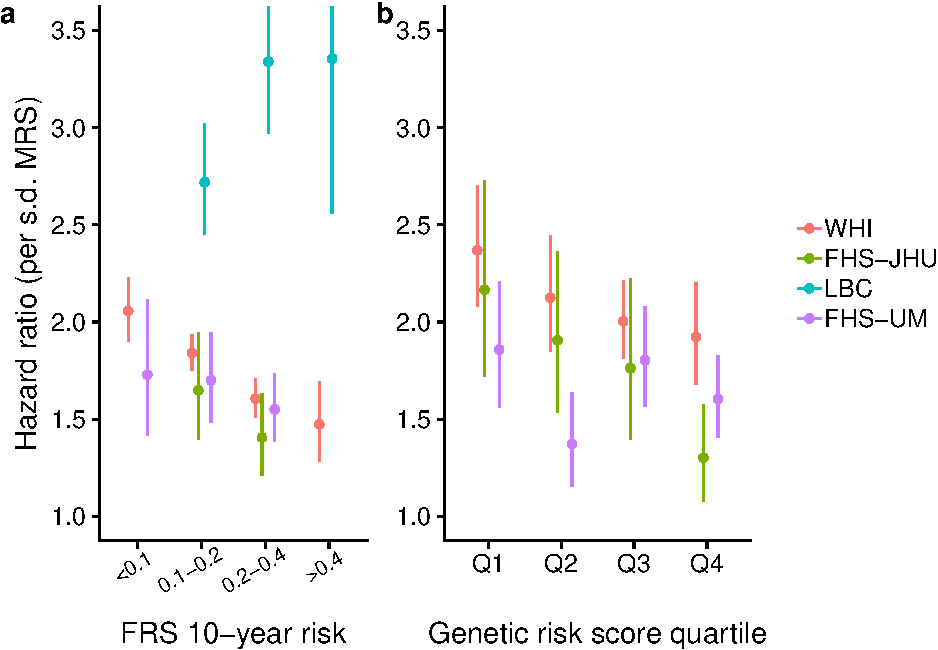
\includegraphics{figures/interactions-1} \caption{Interactions of MRS with other biomarkers of CVD risk. a) Hazard ratios for the MRS within subsets of 10-year generalized CVD risk according to the Framingham Risk Score. b) Hazard ratios for the MRS within quartiles of a genetic cardiovascular risk score (in white participants only for WHI). Hazard ratios are estimated using the final MRS, which was trained using each of these datasets. Stratum-specific Cox regressions were adjusted for age, sex, and estimated cell subtype fractions. Estimates for strata with less than 25 incident events are not shown. Error bars represent standard errors for the hazard ratio estimates (cut off above in panel (a) for ease of visualization of other points).}\label{fig:interactions}
\end{figure}


\end{document}
